%%%%%%%%%%%%%%%%%%%%%%%%%%%%%%%%%%%%%%%%%%%%%%%%%%%%%%%%%%%%%%%%%%%%%%%%%%%%%%%
% Chapter 4 : Título del Capítulo cuatro
%%%%%%%%%%%%%%%%%%%%%%%%%%%%%%%%%%%%%%%%%%%%%%%%%%%%%%%%%%%%%%%%%%%%%%%%%%%%%%%
\section{Descripción de las Funciones Propuestas por el GenOpt}
\label{sec:GENOPT}

El concurso \textit{GenOpt} ha propuesto un total de \textbf{18 funciones} de dimensiones $D = 10, 30$ a optimizar. A partir de sus características, estas funciones se pueden agrupar en tres familias diferentes: 

\bigskip
\subsection{Funciones GKLS}\label{sec:GKLS}
Las funciones GKLS \cite{GKLS} son obtenidas mediante un generador de funciones de tres tipos (no-diferenciable, continuamente diferenciable y dos veces continuamente diferenciable) con mínimos locales y globales conocidos.
 
\subsection{Funciones clásicas transformadas}

Esta familia de funciones se obtienen realizando una transformación a aquellas funciones clásicas para probar métodos de optimización global continua como son:
    \begin{itemize}
    	\item Rastrigin, $D = 10, 30$ \\
    		\begin{equation}\label{eq:rastrigin}
					f(x) = An + \sum^{d}_{i=1}{[x^{2}_{i} - A \cos{2\pi x_{i}}]}
 					\end{equation}
    	\item Rosenbrock, $D = 10, 30$ \\
    	    \begin{equation}\label{eq:rosenbrock}
					f(x,y) = (a - x)^{2} + b(y - x^{2})^{2}
 					\end{equation}
    	\item Zakharov, $D = 10, 30$ \\
    	    \begin{equation}\label{eq:zakharov}
					f(x) = \sum^{d}_{i=1}{x_{i}^{2}} + (\sum^{d}_{i=1}{0.5ix_{i}})^{2} + (\sum^{d}_{i=1}{0.5ix_{i}})^{4}
 					\end{equation}
    \end{itemize}
    Cada función \textit{x} es transformada en cada instancia de la siguiente manera: 
    \begin{equation}
    x' = Mx + x_{0}
    \end{equation}
    Dónde $x_{0}\in[-0.1, 0.1]^{D}$ es un translación aleatoria y M es una matriz ortogonal con número de condición igual a 100.

\subsection{Funciones compuestas} 

Por último, en esta familia encontraremos funciones obtenidas a partir de la composición de las funciones de la segunda familia. Estas funciones se construyen seleccionando aleatoriamente \textit{n} funciones clásicas $f_{1},...,f_{n}$ del siguiente conjunto: 
    	  \begin{itemize}
    	  	\item Goldstein-Price, $D_{f} = 2$;
    	  	\item Hartmann, $D_{f} = 3; 6;$
    	  	\item Rosenbrock, $D_{f} = rand(3, D/2);$
    	  	\item Rastrigin, $D_{f} = rand(3, D/2);$
    	  	\item Sphere, $D_{f} = rand(3, D/2);$
    	  	\item Zakharov, $D_{f} = rand(3, D/2);$
    	  \end{itemize}
    La suma de las dimension $D_{f_{1}},...,D_{f_{n}}$ debe cumplir que $\sum_{i}{D_{f_{i}}} = D$. \\
    Una función \textit{x} es sujeta a un roto-translación tal que, para cada instancia: 
    \begin{equation}
    	x' = Ux + X_{0}
    \end{equation}
    Dónde $U$ es una matriz ortogonal aleatoria y $x_{0}\in[-0.1, 0.1]^{D}$ es una pequeña translación aleatoria. El valor de cada instancia es calculado como: 
    \begin{equation}
    	f(x) = c + \sum^{n}_{i=1}{f_{i}(x'_{b_{i}},...,x'_{b_{i}} + D_{f_{i}} - 1)}
    \end{equation}
    Dónde $b_{i} = \sum^{i-1}_{j=1}{D_{f_{i}}}$. \\
    En la siguiente figura podemos observar un esquema de este proceso: 
    	  \begin{figure}[!ht]
  				\centering
					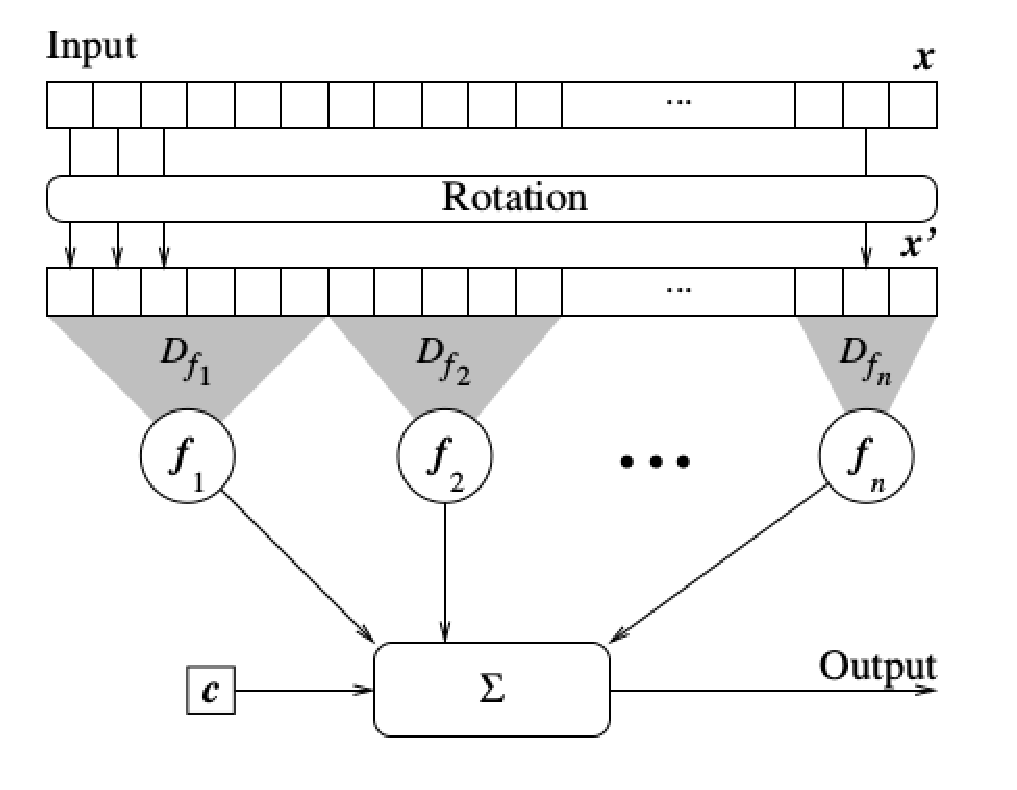
\includegraphics[scale=0.5]{images/composicion}
  				\caption{Composición de funciones.}
				\end{figure}

\newpage

%%%%%%%%%%%%%%%%%%%%%%%%%%%%%%%%%%%%%%%%%%%%%%%%%%%%%%%%%%%%%%%%%%%%%%%%%%%%%%
\section{Estudio de la Parametrización}\label{sec:PARAM}

En esta sección trataremos el estudio de los parámetros empleados por cada uno de los algoritmos y como afectan al desempeño de los mismos. \\

Un parámetro común a todos los algoritmos desarrollados es el tamaño de la población, y es por ello que, se empleará para contrastar el desempeño de los mismos hemos realizado experimentos con tamaños de población o $popsize = 20, 50, 75, 100$, a excepción del algoritmo SA (sección \ref{sec:SA}) que debido a que se trata de una meta-heurística de trayectoria se empleará únicamente un individuo.

\subsection{OBL-CPSO}\label{sec:paramOBL_CPSO}

En el diseño del algoritmo OBL-CPSO (sección \ref{sec:OBL-CPSO}) sólo se contempla la utilización de un parámetro, el tamaño de población. Es por ello, que los experimentos realizados con este algoritmo buscan encontrar el tamaño de población más adecuado para su rendimiento. A continuación, podemos ver una comparativa de los experimentos realizados con $popsize = 20, 50, 75, 100$: \\

\begin{figure}[!ht]
  \centering
	%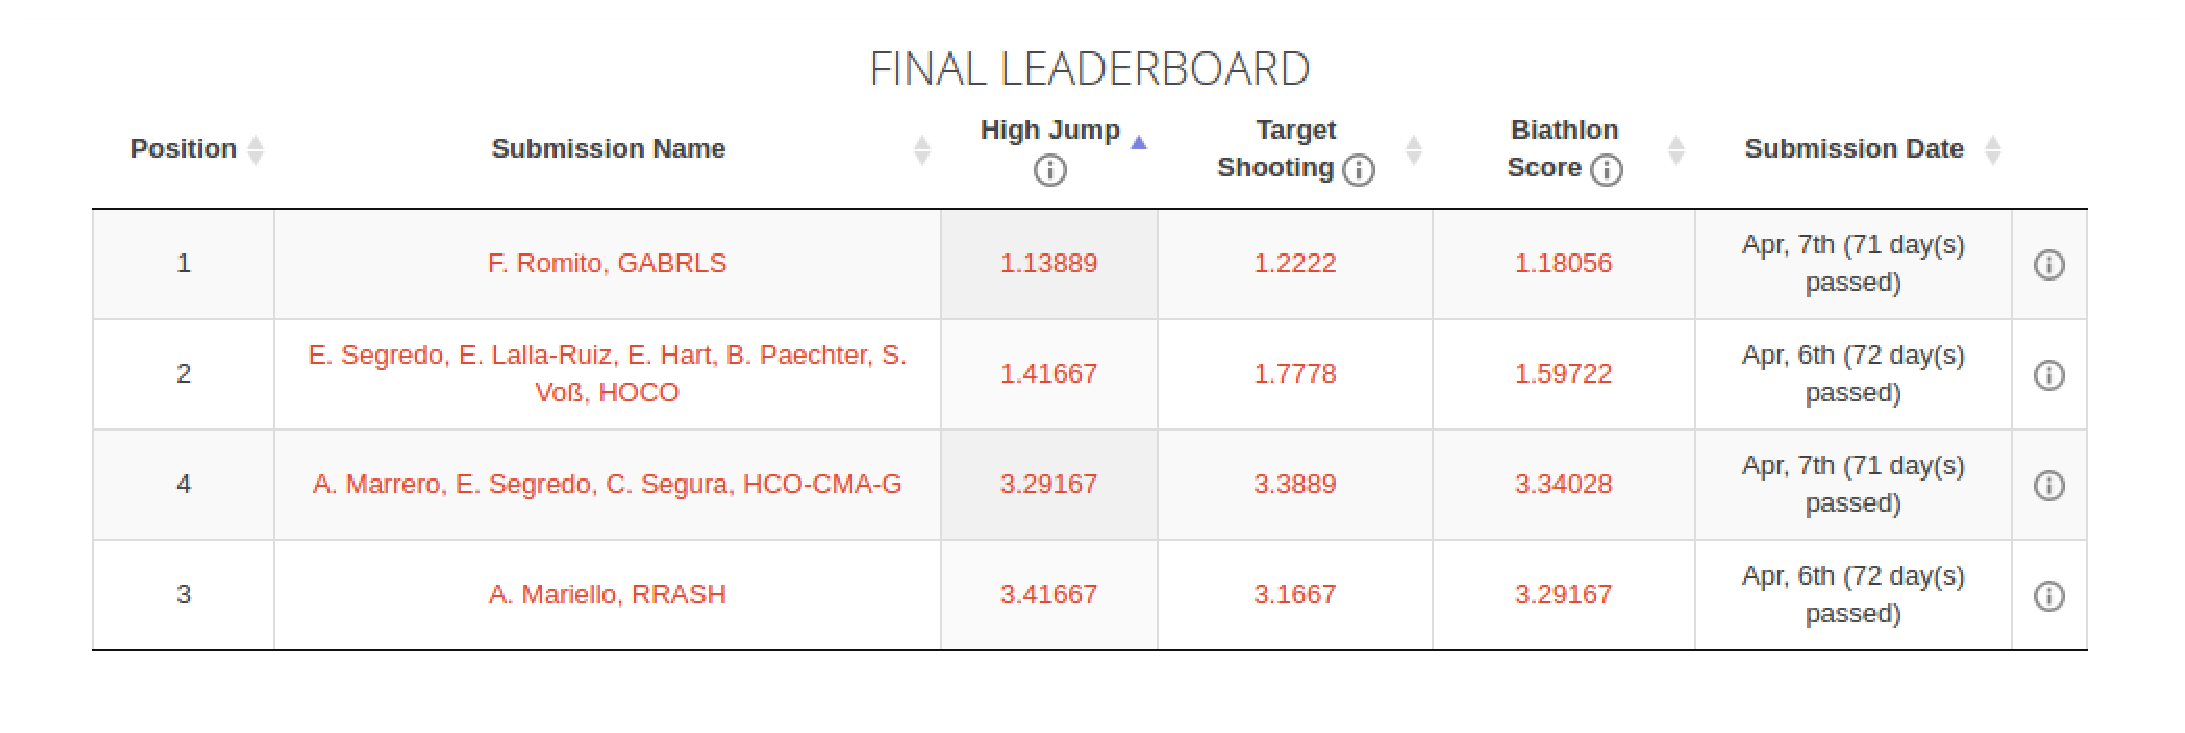
\includegraphics[scale=0.5]{images/final}
	\captionsetup{justification=centering}
  \caption{Comparativa del algoritmo OBL-CPSO con diferentes tamaños de población.}
\end{figure}

\subsection{CMA-ES}\label{sec:paramCMA_ES}

El diseño del algoritmo CMA-ES, como detallamos en la sección \ref{sec:CMA}, sólo necesita la definición de dos parámetros iniciales para comenzar su ejecución, el tamaño de la población a emplear y el valor de sigma ($\sigma$) inicial. \\
El tamaño de la población, como especificamos en el inicio de la sección, tomará los siguientes valores $popsize = 20, 50, 75, 100$. \\
En cuanto al parámetro $\sigma$, los valores que tomará serán $\sigma = 0.3, 0.8, 2.0$. La elección de estos valores se basa en que el parámetro $\sigma$ determina la variación incluida en cada nueva generación de la población y teniendo en cuenta esto, unos valores de $\sigma$ pequeños como 0.3 y 0.8 harán que el algoritmo se comporte como una búsqueda local, y al contrario con valores grandes de $\sigma$ como 2.0 \cite{CMA1}. \\

Para evaluar el rendimiento del algoritmo variando estos dos parámetros, hemos realizado un total de 12 experimentos, obteniendo los siguientes resultados:

\begin{figure}[!ht]
  \centering
	%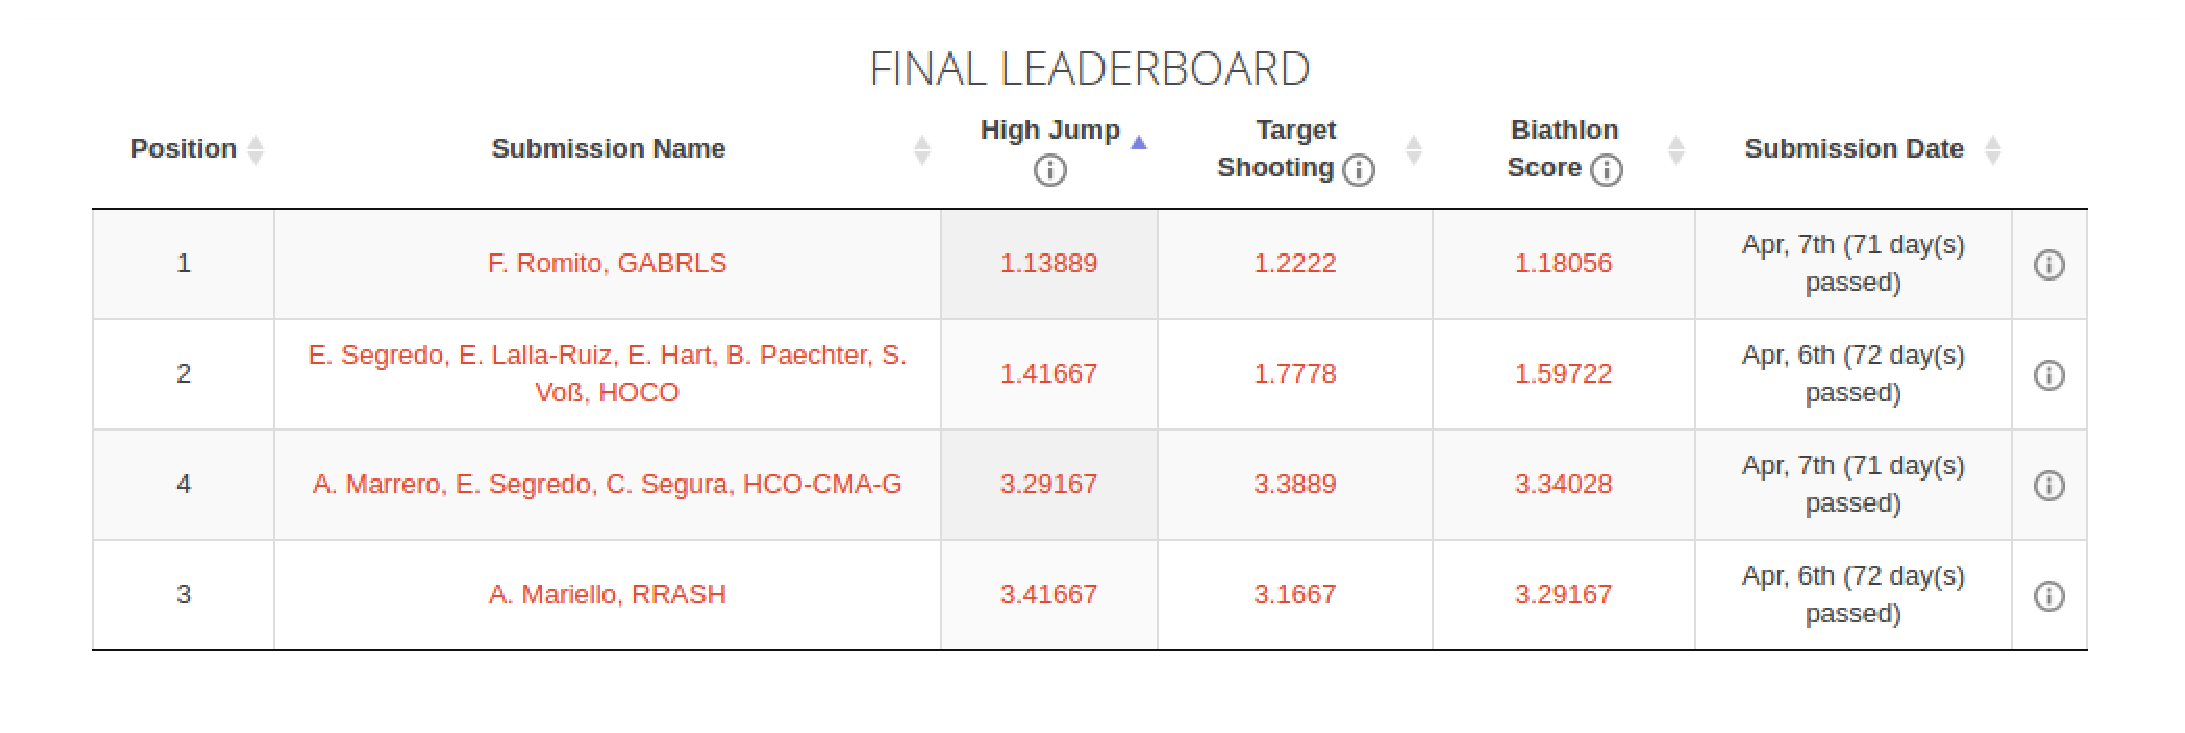
\includegraphics[scale=0.5]{images/final}
	\captionsetup{justification=centering}
  \caption{Comparativa del algoritmo CMA-ES.}
\end{figure}

\subsection{SA}\label{sec:paramSA}

Por último, el algoritmo SA (sección \ref{sec:SA}) presenta únicamente un parámetro, la temperatura inicial. Según la literatura \cite{metabook}, inicialmente este parámetro debe tener un valor elevado, y es por ello, por lo que los valores con los que hemos evaluado el rendimiento de este algoritmo han sido $Temp_{0} = 500, 1000, 10000$. A continuación, podemos ver una comparativa de los resultados obtenidos. 

\begin{figure}[!ht]
  \centering
	%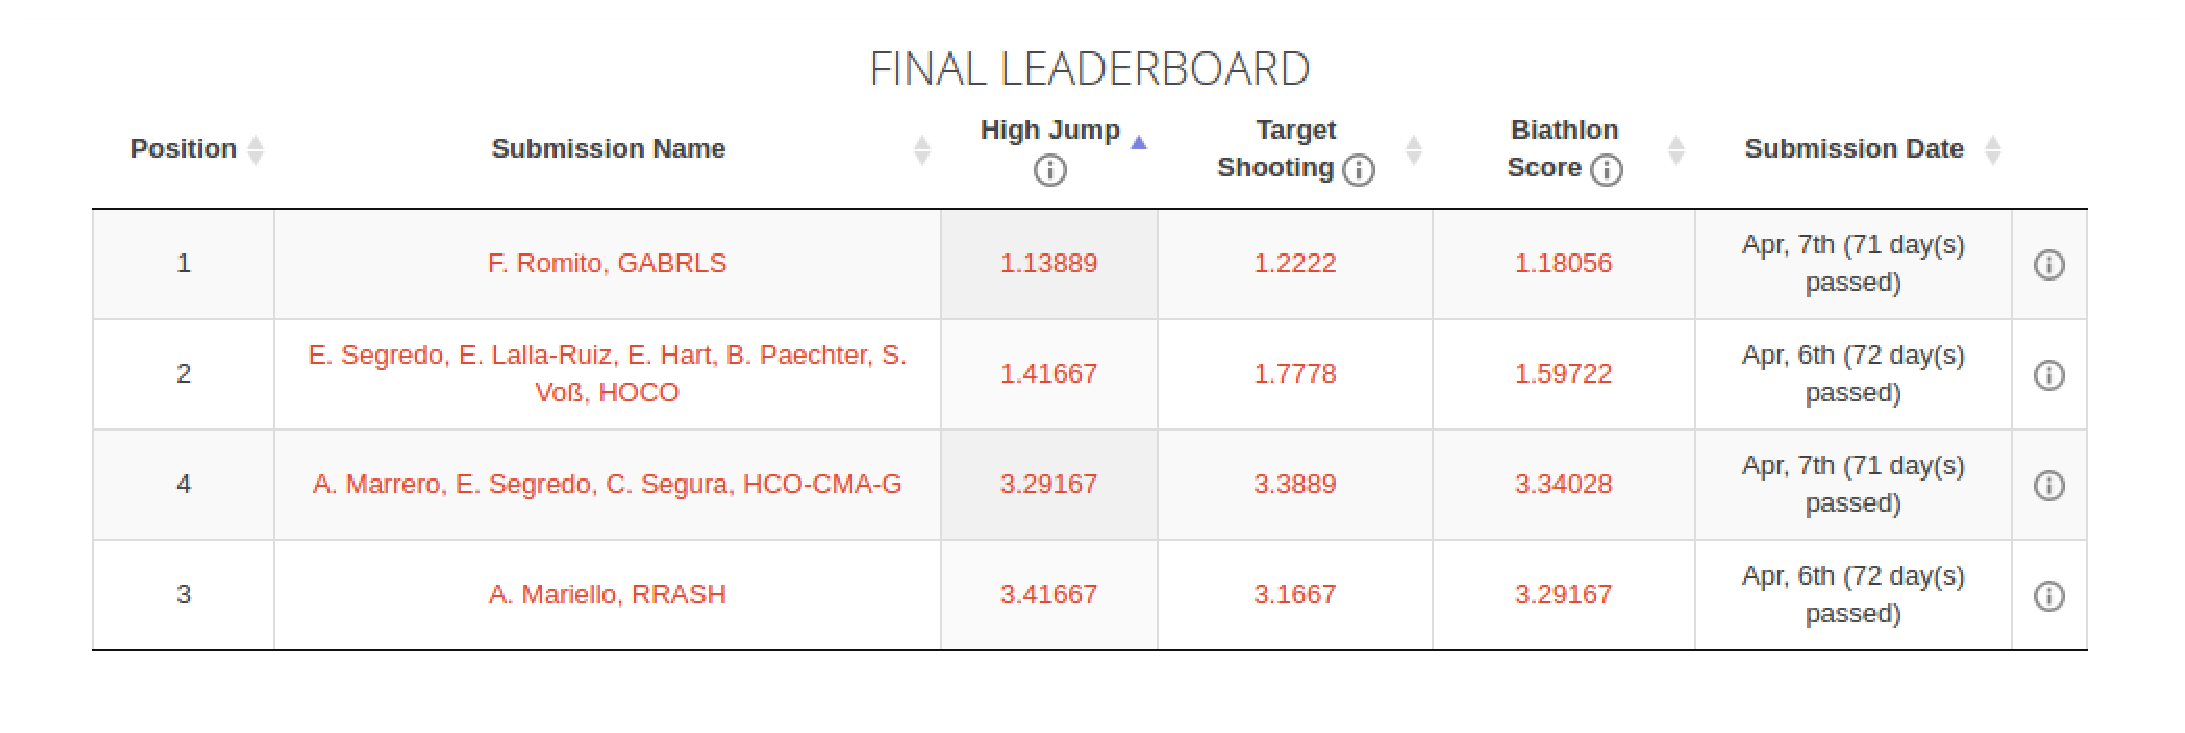
\includegraphics[scale=0.5]{images/final}
	\captionsetup{justification=centering}
  \caption{Comparativa del algoritmo SA con diferentes valores de temperatura inicial.}
\end{figure}

%%%%%%%%%%%%%%%%%%%%%%%%%%%%%%%%%%%%%%%%%%%%%%%%%%%%%%%%%%%%%%%%%%%%%%%%%%%%%%
\section{Análisis de Rendimiento}\label{sec:PERFORMANCE}


%%%%%%%%%%%%%%%%%%%%%%%%%%%%%%%%%%%%%%%%%%%%%%%%%%%%%%%%%%%%%%%%%%%%%%%%%%%%%%
\section{Clasificación en el Concurso GenOpt}\label{sec:Competition}

Desde la organización del concurso GenOpt proponen varios criterios para clasificar los algoritmos enviados por los participantes. Estos criterios pueden ser:

\begin{itemize}
    	  	\item \textbf{High Jump}: Mejor valor obtenido en los puntos de control.
    	  	\item \textbf{Target Shooting}: Éxito a la hora de alcanzar el óptimo global de la función.
    	  	\item \textbf{Biathlon Score}: Media entre el High Jump y Target Shooting.
\end{itemize}

A la vista de los resultados obtenidos en el análisis de rendimiento decidimos emplear el algoritmo CMA-ES (sección \ref{sec:CMA}) para participar en la fase final del concurso. \\
Con este algoritmo, el cual denominamos \textit{Hybrid Continuous Optimiser based on CMA-ES and a Global Neighbourhood Path Search (HCO-CMA-G)}, conseguimos la \textbf{tercera posición} en el ranking final según el parámetro \textbf{High Jump}, como podemos ver en la siguiente figura: 

\begin{figure}[!ht]
  \centering
	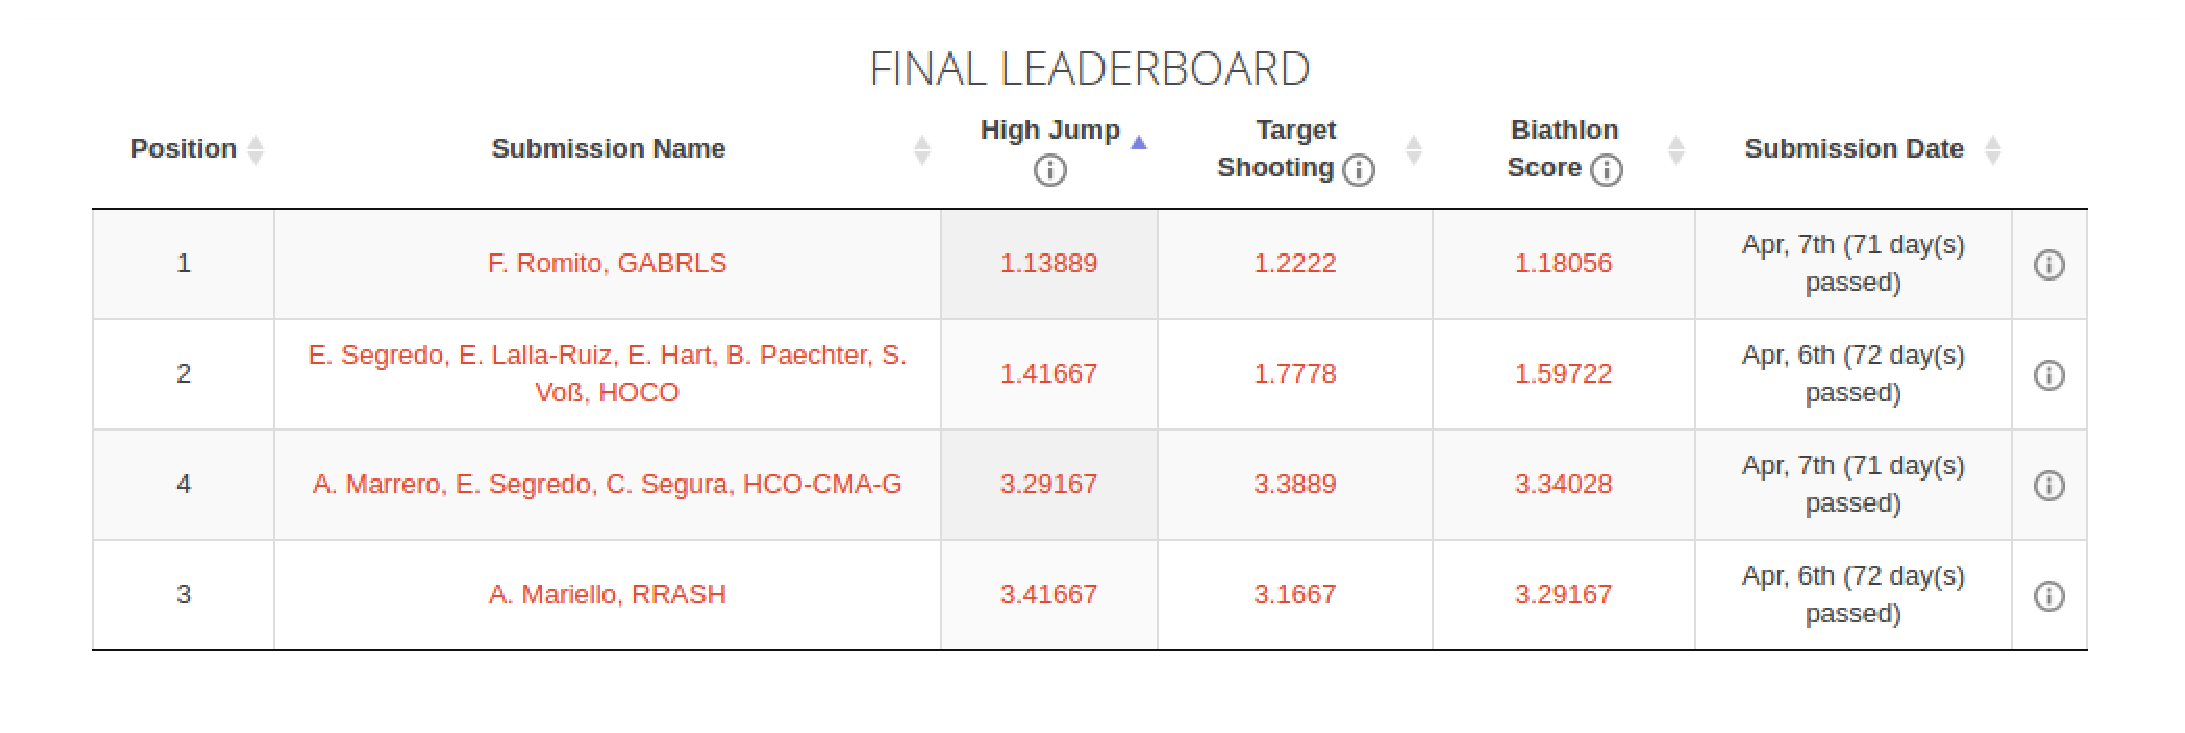
\includegraphics[scale=0.5]{images/final}
  \caption{Clasificación en el concurso GenOpt según High Jump.}
\end{figure}

\newpage